\documentclass{beamer}
\usepackage[english,russian]{babel}
\usepackage[utf8]{inputenc}
\usepackage{amsmath}
\usepackage{hyperref}
\usetheme{Warsaw}
\usepackage{listings}
\usepackage{xcolor}
\usepackage{tikz}
\usetikzlibrary{graphs}
\usepackage{algpseudocode}

\lstset{
    frame=tb,
    tabsize=4,
    showstringspaces=false,
    numbers=left,
    commentstyle=\color{green},
    keywordstyle=\color{blue},
    stringstyle=\color{red},
    emph={baz},
    emphstyle=\textbf
}
\begin{document}

\title{SAT/SMT solvers\newline  9. Deciding a Combination of Theories}
\author{Roman Kholin}
\institute{Lomonosov Moscow State University}
\date{Moscow, 2023}

\begin{frame}
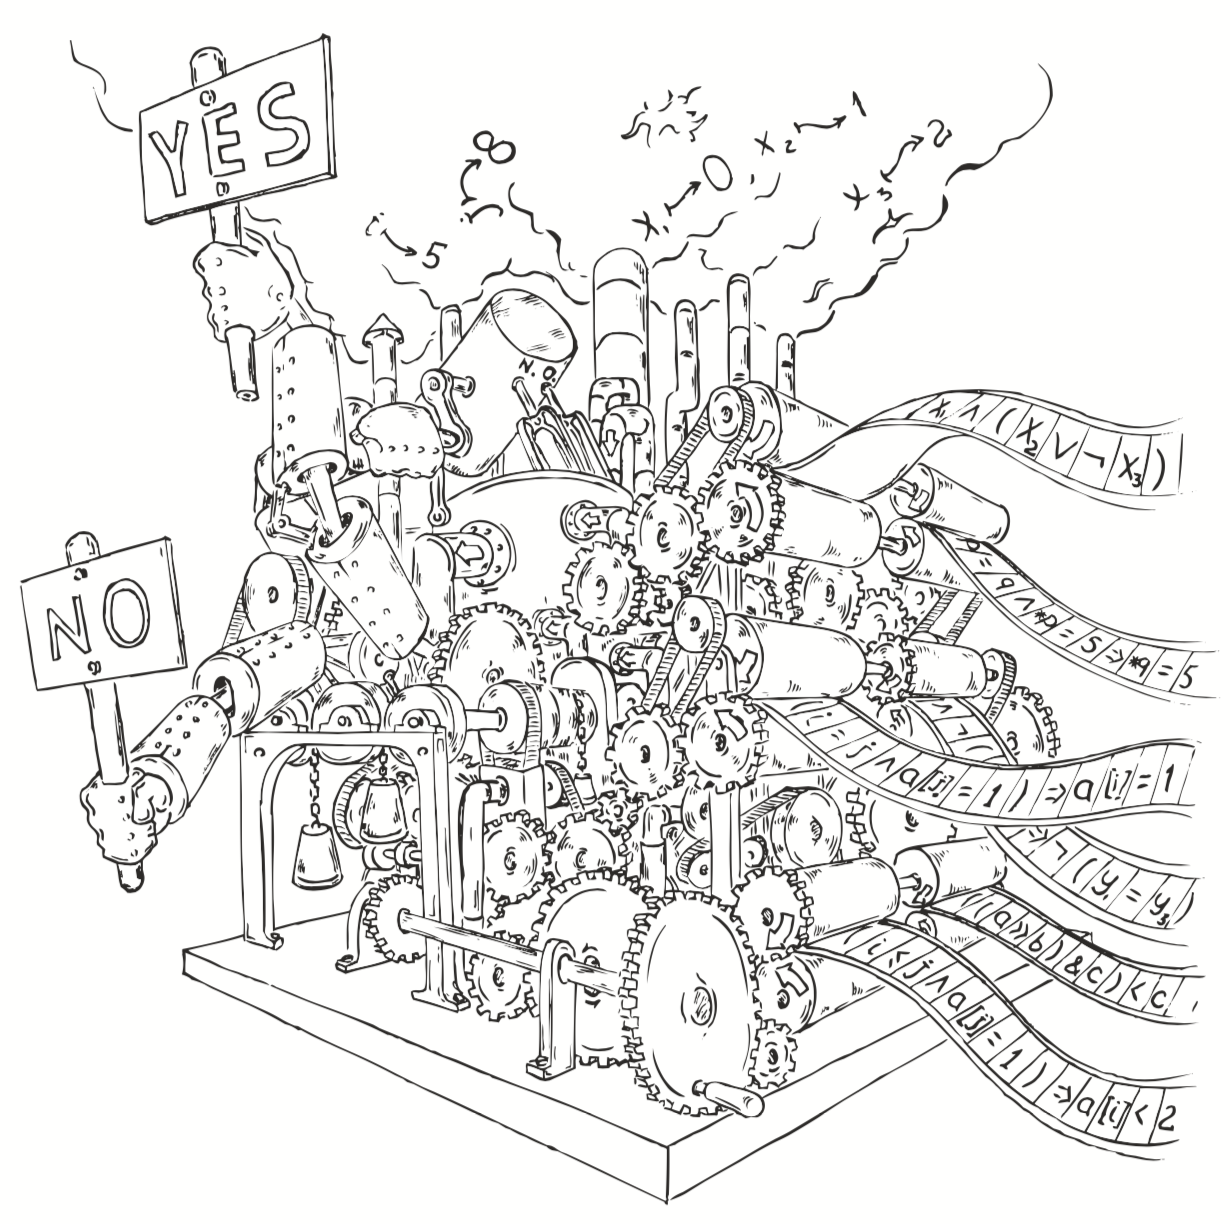
\includegraphics[scale=0.5]{../decision-procedure.png}
\end{frame}

\frame{\titlepage}

\begin{frame}{Why we need it}
\begin{enumerate}
\item A combination of linear arithmetic and uninterpreted functions:\newline
$(x_2 \ge x_1 ) \wedge (x_1 - x_3 \ge x 2 ) \wedge (x_3 \ge 0) \wedge f(f(x_1) - f(x_2)) \ne f(x_3)$
\item A combination of bit vectors and uninterpreted functions:\newline
$f(a[32], b[1]) = f (b[32], a[1]) \wedge a[32] = b[32]$
\item A combination of arrays and linear arithmetic:
$x = v\{i \leftarrow e\}[j] \wedge y = v[j] \wedge x > e \wedge x > y$
\end{enumerate}
\end{frame}

\begin{frame}{Theories}
\begin{enumerate}
\item Variables
\item Logical symbols: $\vee, \wedge, \rightarrow, \lnot$, $\forall, \exists$
\item Nonlogical symbols, namely function and predicate symbols
\item Syntax
\end{enumerate}
\begin{itemize}
\item It is common to consider the equality sign as a logical symbol rather than a predicate
\item Signature $\Sigma$ is a set of nonlogical symbols (i.e., function and predicate symbols)
\item A first-order theory is defined by a set of sentences (first-order formulas in which all variables are quantified) or axioms
\item A $\Sigma$ - formula $\phi$ is $T$-satisfiable if there exists an interpretation that satisfies both $\phi$ and $T$
\item A $\Sigma$-formula $\phi$ is $T$-valid ($T\models\phi$) if all interpretations that satisfy $T$ also satisfy $\phi$
\end{itemize}
\end{frame}

\begin{frame}{Theory combination}
Given two theories $T_1$, $T_2$ with signatures $\Sigma_1$, $\Sigma_2$ respectively, the theory combination $T_1 \oplus T_2$
is a ($\Sigma_1 \cup \Sigma_2$)-theory defined by the axiom set $T_1 \cup T_2$
\end{frame}

\begin{frame}{Convex theory}
$\Sigma$-theory $T$ is convex if for every conjunctive $\Sigma$-formula $\phi$:\newline
$(\phi \implies \vee_{i=1}^{n}(x_i=y_i))$ is $T$-valid for some finite $n > 1 \implies$\newline
$(\phi \implies (x_i=y_i))$ is $T$-valid for some $i \in \{1, \dots, n\}$
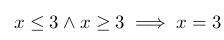
\includegraphics[scale=0.5]{convex.png}\newline
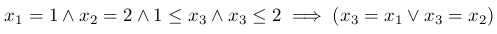
\includegraphics[scale=0.5]{not_convex.png}\newline
\end{frame}

\begin{frame}{Nelson-Oppen restrictions}
\begin{enumerate}
\item $T_1, \dots T_n$ are quantifier-free first-order theories with equality
\item There is a decision procedure for each of the theories
\item The signatures are disjoint
\item Theories that are interpreted over an infinite domain
\end{enumerate}
\end{frame}

\begin{frame}{Purification}
Let $\phi' := \phi$
\begin{enumerate}
\item For each "alien" subexpression $\varphi$ replace on $a_{\varphi}$
\item Constrain $\phi'$ with  $a_{\varphi} = \varphi$
\end{enumerate}
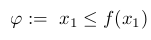
\includegraphics[scale=0.5]{ex1.png}\newline
After purification, we are left with a set of pure expressions $F_1, \dots, F_n$, such that:
\begin{enumerate}
\item For all $i$, $F_i$ belongs to theory $T_i$ and is a conjunction of $T_i$-literals
\item Shared variables are allowed
\item The formula $\phi$ is satisfiable in the combined theory if and only if $\wedge_{i=1}^{n}F_i$
\end{enumerate}
\end{frame}

\begin{frame}{Nelson-Oppen for Convex Theories}
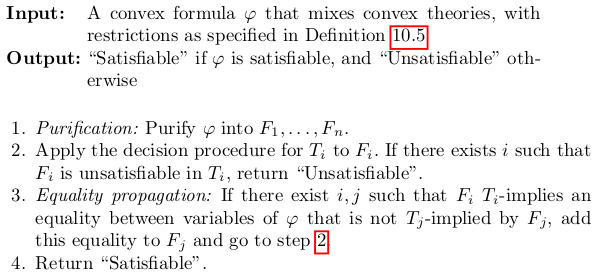
\includegraphics[scale=0.5]{Nelson-Oppen-for-Convex-Theories.png}\newline
\end{frame}

\begin{frame}{Example}
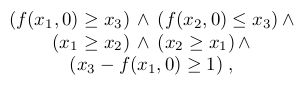
\includegraphics[scale=0.5]{ex2.png}\newline
\end{frame}

\begin{frame}{Example}
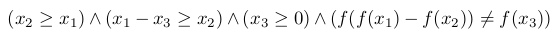
\includegraphics[scale=0.5]{ex3.png}\newline
\end{frame}

\begin{frame}{Nelson-Oppen}
Algorithm may fail if one of the theories is not convex:
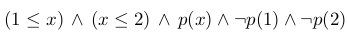
\includegraphics[scale=0.5]{ex4.png}\newline
\end{frame}

\begin{frame}{Nelson-Oppen}
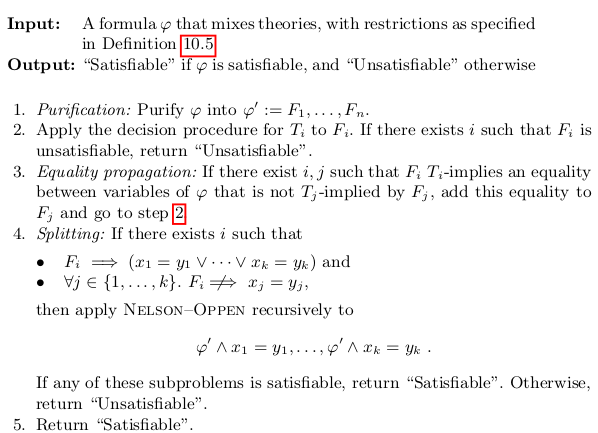
\includegraphics[scale=0.5]{Nelson-Oppen.png}\newline
\end{frame}

\begin{frame}{Example}
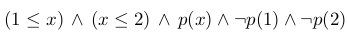
\includegraphics[scale=0.5]{ex4.png}\newline
\end{frame}

\begin{frame}
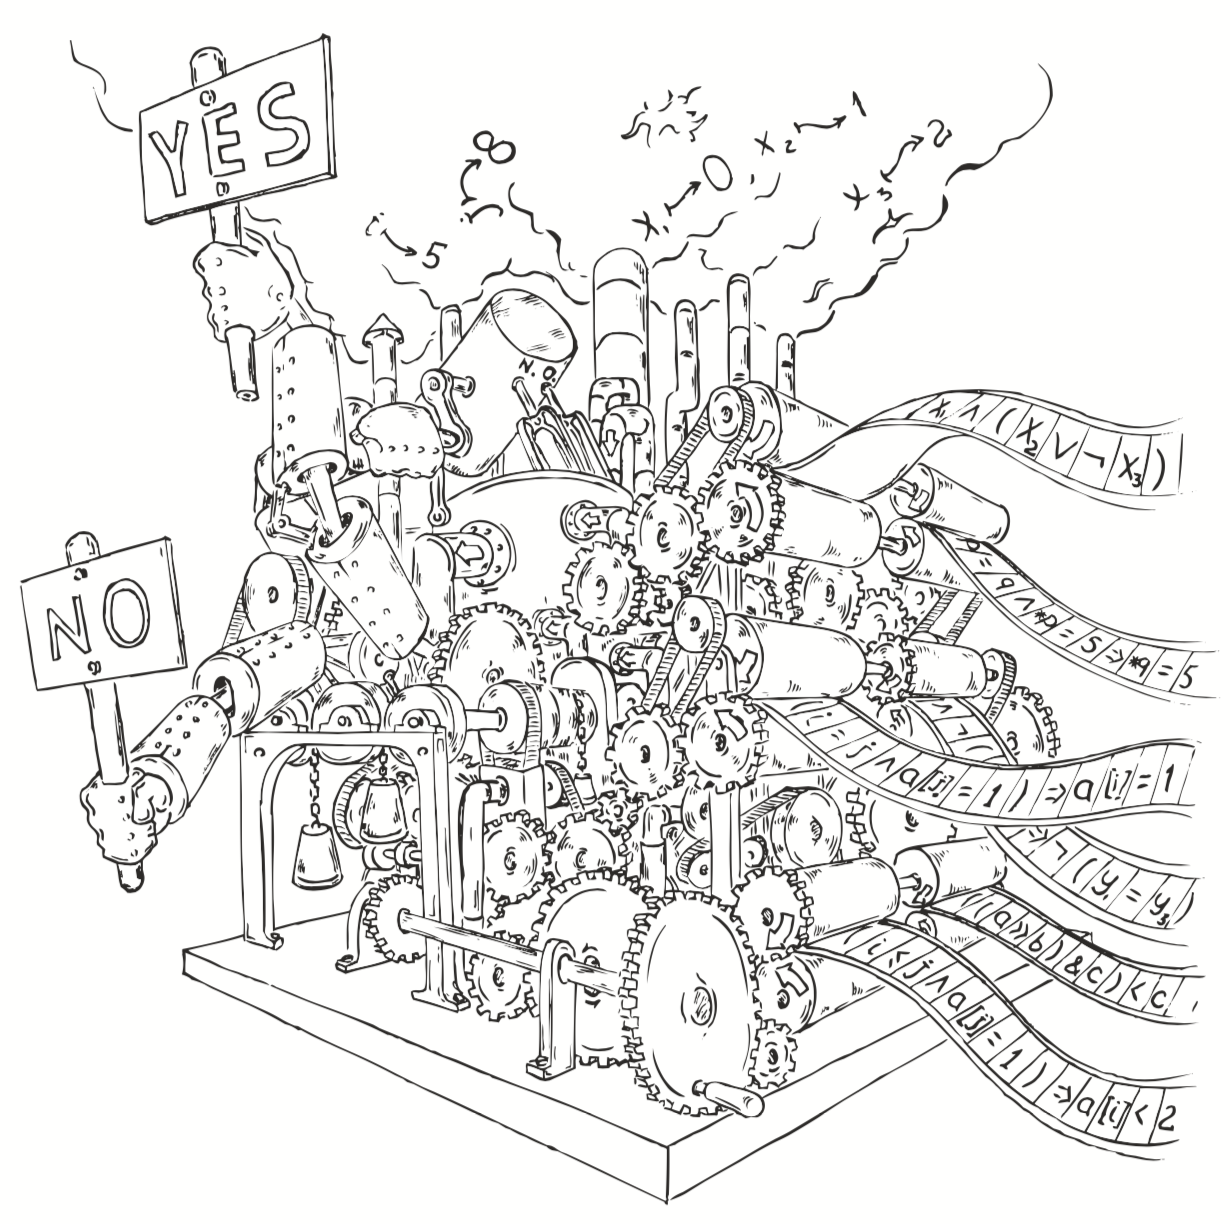
\includegraphics[scale=0.5]{../decision-procedure.png}
\end{frame}

\end{document}
